\chapter{Benchmarks}

In this chapter, we show the difference between using \texttt{PhpTreeBuilder} properly and only the \texttt{AddMarkupContent} method.
Then, we test the speed of three PHP library functions in the Blazor and desktop environments.
These benchmarks are available as .NET solutions in the attachment.
We introduce the background of the benchmarks, execute them and then evaluate the results.
\par
The tests were executed on a HP Spectre x360 Convertible laptop with Intel(R) Core(TM) i7-8550U CPU, 8GB RAM, and NVIDIA GeForce MX150.
They used Google Chrome (version: 90.0.4430.93) browser and Apache server.

\section{Rendering}

This benchmark observes the refreshing speed of a page using two ways for rendering a page content.
We modify the \texttt{Asteroids} game, mentioned earlier, to explore FPS during rendering.
The modified application generates asteroids, represented by \texttt{<div>} element with CSS styles, and lets them fall until they reach the bottom, as we can see in Figure \ref{img33:benchmark}.
Then, they are removed.
We log the current FPS, count of elements generated by the application, and time from starting the measurement every second.
Then, we evaluate the results.
\par
\begin{figure}[t]\centering
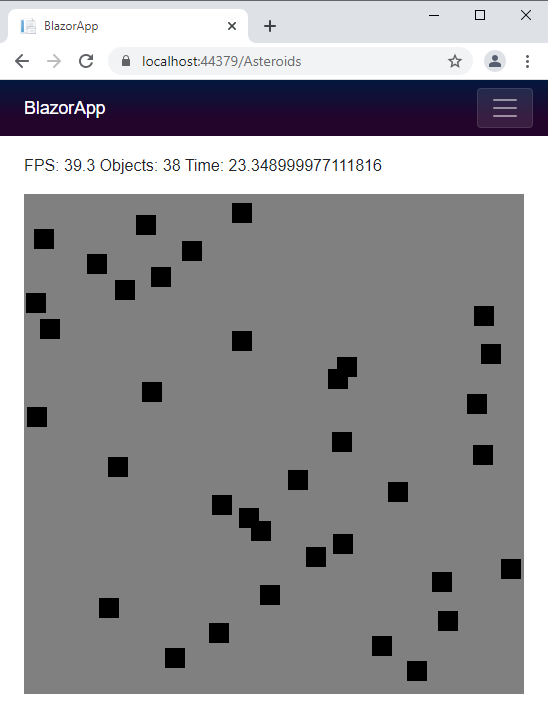
\includegraphics[scale=0.7]{./img/BenchmarkRendering}
\caption{The benchmark counts the number of frames per second. At the top of the figure, we can see the current FPS, the number of HTML tags in the game, and elapsed seconds from the game beginning.}
\label{img33:benchmark}
\end{figure} 
\par
The .NET solution comprises three projects: \texttt{BlazorApp.Client}, \texttt{BlazorApp.Server}, \texttt{PHPScripts}.
The setting of BlazorApp is similar to the previous examples.
\texttt{PHPScripts} contains the modified game together with additional scripts providing the interactive setting for the benchmark in a browser.
When we start the server and navigate the website, we can set various properties of measurement like an upper bound of FPS, a frequency of asteroids, or dimensions of background.
We will explain only the \textit{Rendering} property because the rest of the properties are self-explanatory.
We have two options for the property.
We call the first one \texttt{String} rendering because it uses \texttt{AddMarkup} method for updating the page content.
This method accumulates the generated HTML entities into a single string and adds it into \texttt{PhpTreeBuilder}.
We call the second one \texttt{Diff} rendering because it utilizes specialized builder interface for adding HTML entities, which includes \texttt{AddAttribute} for example.
\par
We suppose that the first method is less effective than the second because the diff algorithm makes lesser update optimizations in the first case.
It is caused by not providing the sequence numbers for each of the HTML entities, but it is regarded as the one part.
This method simulates the rendering of a whole script by \texttt{PhpScriptProvider}, which obtains the script output as a string and passes it to the \texttt{AddMarkupContent} method.
This part is regenerated every time instead of update only the changed parts.
We measured FPS 10 times for each configuration and then made a mean of them.
Data of these measurements can be found in the attachment.
\par
We can see results from the first measurement in Figure \ref{img31:benchmark1}, which uses one tag element representing an asteroid.
We set the timer to refresh the window in one-thousandth of a second after building the rendering tree.
The resulting speed will be significantly lower, but we want to measure the maximum rendering speed of Blazor, which can be done by almost immediately waiting for the next rendering. 
We generate five asteroids per second.
The dimensions of the background are 800 x 800.
We measure the FPS and number of objects for 60 seconds.
We can see a graph displaying the current FPS and number of objects.
The lines represent measured values for each type of rendering.
In spite of mean, the lines are not smooth.
It is caused by a difference of a sampling rate, where the measurements do not log FPS in the common numbers of objects.
But we think that the graphs sufficiently prove our hypothesis.
\par
The second measurement aims at the deeper structure of updating elements in Figure \ref{img32:benchmark2}.
The setting is the same as the previous one.
\par
\begin{figure}\centering
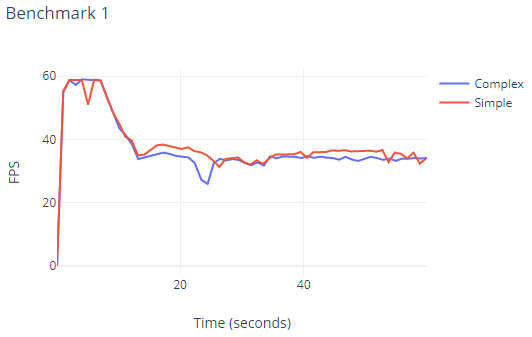
\includegraphics{./img/graph_1}
\caption{The graph represents measured FPS for the current number of objects, where we use only a single tag for an asteroid. The \textit{Diff} method uses \texttt{PhpTreeBuilder} properly. The second method simulates rendering by \texttt{PhpScriptProvider}, where a script output is passed into the \texttt{AddMarkupContent} method.}
\label{img31:benchmark1}
\end{figure} 
\par
\begin{figure}\centering
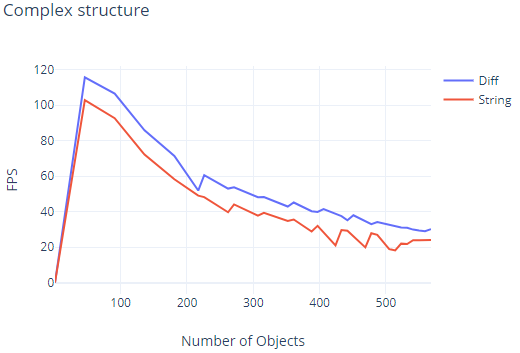
\includegraphics{./img/graph_3}
\caption{The graph represents measured FPS for the current number of objects, where we use the complex structure of HTML tags for an asteroid.}
\label{img32:benchmark2}
\end{figure} 
\par
We can see that the number of objects was changing during the application runtime.
It is because of the beginning state of the application, where there are no asteroids.
When the first asteroids fell to the bottom, the number was stable.
We can see that when the updating objects had not inner elements, the rendering ways were the same at the end of the graph.
When the updated objects had inner elements, the FPS was lower in the first way of rendering, as we can see in Figure \ref{img32:benchmark2}.
This is caused by optimized updates made by the diff algorithm, which generates only DOM updates for the element style and leaves the inner tree unchanged.
As we can see, the FPS was about 30 in a second way when the number of asteroids was stable, which is fine because the untrained eye is able to distinguish up to 23 images per second.
The first way had about 24 FPS, which looked glitchy in the browser.
This benchmark demonstrates when it is a good choice to use the builder properly and the need to use \texttt{PhpComponent} for render demanding applications.
\par
Another problem caused by the first way of rendering is handling click events when the window is being quickly refreshed.
Because the click events consist of two inner events (mouse up, mouse down), the event is not fired due to removing the element before the second event appears.

\section{Performance of libraries}

This benchmark wants to highlight performance of PHP libraries in the Blazor environment.
We prepared a simple script, which measures execution time of the following three functions: \texttt{imagecreatetruecolor}, \texttt{str\_getcsv}, \texttt{md5}.
The first function creates a 1920x1080 blank image.
The second function converts a short string representing CSV data to an array.
The last function computes a hash of the CSV string.
We measure elapsed time during the function execution multiple times and then make a mean.
This approach should make the time spend with the JIT compilation less important.
We compare the results of executing the script in a desktop environment, where we use Peachpie, the Blazor environment using Peachpie as well, and the native PHP interpreter.
\par
The benchmark is created as a .NET solution consisting of four projects: \texttt{BlazorApp.Client}, \texttt{BlazorApp.Server}, \texttt{Desktop}, \texttt{PHPScripts}.
The \texttt{PHPScripts} project contains \textit{index.php}, which does the benchmark.
The \texttt{Desktop} project runs the script in a console application.
\texttt{BlazorApp} projects run the script in a browser.
\par
\begin{table}[b!]
\centering
\begin{tabular}{l@{\hspace{1.5cm}}D{.}{,}{2.0}D{.}{,}{2.0}D{.}{,}{2.0}}
\toprule
\textbf{Environment} & \mc{\textbf{imagecreatetruecolor}} & \mc{\textbf{str\_getcsv}} & \mc{\textbf{md5}}\\
\midrule
Blazor - Peachpie  & \mc{\num{23e6}} &  \mc{60} & \mc{Error} \\
Desktop - Peachpie & \mc{\num{2e4}} & \mc{1.9} & \mc{1.8} \\
Desktop - Native   & \mc{\num{5e2}} & \mc{7.2} & \mc{\num{0.4}} \\
\bottomrule
\end{tabular}
\caption{Elapsed time (microseconds) of the function executions.}
\label{tab01:time}
\end{table}
\par
We can see the result of measurement in Table \ref{tab01:time}.
The first observation is the call of the \texttt{md5} function caused an error: \textit{This function is unsupported in this platform}.
The second observation is an extremely slow execution of the \texttt{imagecreatetruecolor} function in the Blazor environment.
We suppose that it is caused by the \texttt{ImageSharp} library, which has not to be optimized in the browser environment.
The difference between the execution times with the PHP interpreter and the console application is caused by using the different libraries.
Peachpie uses libraries, which are written in C\#.
The PHP interpreter uses different libraries written in C.
We can not say that Peachpie or the PHP interpreter is faster due to the results.
\par
This benchmark reveals the need to test a library before it is being used in the Blazor environment.
We suppose that these issues with speed and the error will be solved because Peachpie uses a standard library for the encryption and \texttt{ImageSharp} for the graphics, which has a big community.
On the other hand, if the execution time will be slower than the execution with the PHP interpreter, it would consume a client resource, which is a server benefit.